A Passive Daytime Radiative Cooling (PDRC) device operates by absorbing a lower amount of blackbody radiation than it emits, thereby facilitating electricity-free cooling, even in daylight conditions. Consequently, one of the pivotal attributes of a PDRC device is the imperative for an absorptivity ($\alpha$) as close to 0\% or, conversely, a reflectivity ($R$) of 100\% within the solar spectrum (ranging from 0.3 to 2.5 micrometers). This specification ensures that the device's surface remains entirely unaffected by solar heating during daylight hours.

To enhance the effectiveness of PDRC, it becomes essential to accurately measure and optimize this reflectivity ($R$) within the solar spectrum. One approach for achieving this goal is to perceive light as an electromagnetic wave, and from this perspective, derive a quantifiable means to measure $R$ through the renowned \textit{Fresnel equations}.

The Fresnel equations are mathematical expressions that delineate the proportion of incident energy that is either transmitted or reflected at the interface of two materials with differing refractive indices. This concept aligns precisely with our objectives, as we plan to stack plane surfaces featuring distinct reflective properties and refractive indices. This chapter serves as an exploration of the theoretical framework underpinning the derivation of $R$ via the Fresnel Equations, delving into associated phenomena such as total internal reflection. Additionally, we explore the practical application of these principles to PDRC devices.


\section{Fresnel Equations}
Consider a light ray incident at point P upon a planar interface, leading to the generation of both reflected and refracted rays. It is noteworthy that the refractive index at the interface for both the incident and reflected rays ($n_1$) differs from the refractive index associated with the refracted ray ($n_2$). The plane of incidence lies within the x-z plane and is defined by both the surface normal and the incident ray.

In the context of each ray, the direction of wave propagation ($\vec{\mathbf{k}}$), can be established by the vector cross product of the electric field ($\vec{\mathbf{E}}$), and magnetic field ($\vec{\mathbf{B}}$) vectors, expressed as $\vec{\mathbf{E}} \times \vec{\mathbf{B}}$. This relationship can be conveniently determined using the right-hand rule, offering a valuable method for directional assessment.

% inserting the TE wave example
\begin{figure}
  \centering
  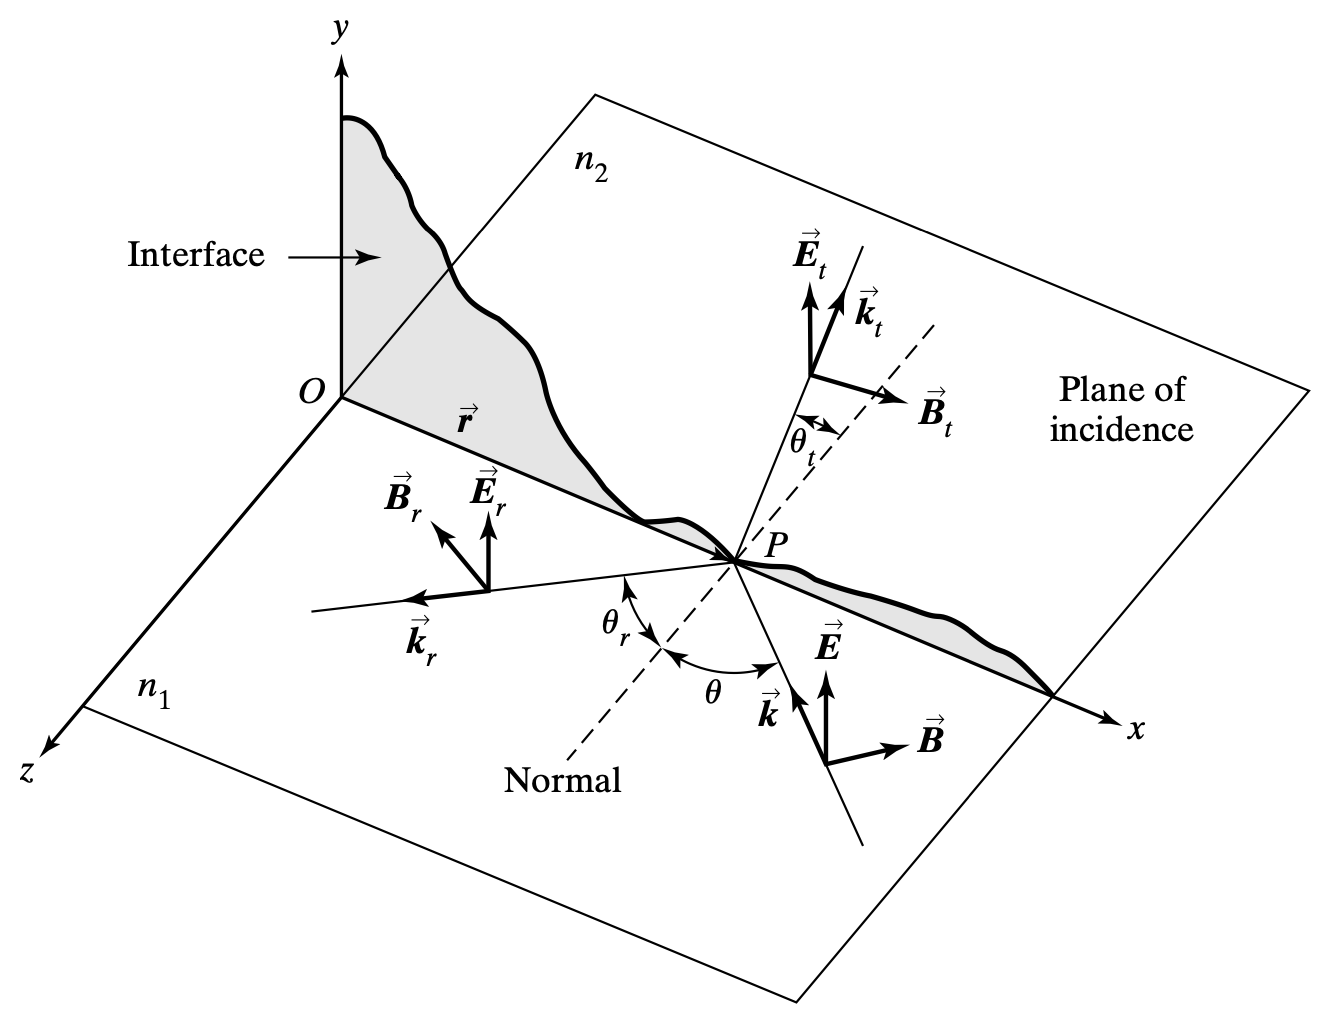
\includegraphics[width=0.8\textwidth]{Chapters/Figures/Incident, Relfected, and Transmitted Ray for TE Mode.png}
  \caption{The transverse electric (TE) set-up}
\end{figure}

Let us consider that the incident light comprises of plane harmonic waves:
\begin{equation} \label{Plane harmonic wave equation - incident}
\vec{\mathbf{E}} = \vec{\mathbf{E}_0} e^{i(\vec{\mathbf{k}} \cdot \vec{\mathbf{r}} - \omega t)}
\end{equation}
In our analytical approach, we will specifically examine a linearly polarized light wave, where the electric field vector $\vec{\mathbf{E}}$ is oriented perpendicular to the plane of incidence. According to the right-hand rule, this configuration places the magnetic field vector $\vec{\mathbf{B}}$ within the plane of incidence. This particular polarization is known as the \textit{transverse electric} (TE) mode

% REPHRASE DOWN ONWARDS
The reflected and transmitted waves can then also be expressed as plane harmonic wave equations:
\begin{equation} \label{Plane harmonic wave equation - reflected}
\vec{\mathbf{E}_r} = \vec{\mathbf{E}_{0r}} e^{i(\vec{\mathbf{k_r}} \cdot \vec{\mathbf{r}} - \omega_r t)}
\end{equation}

\begin{equation} \label{Plane harmonic wave equation - refracted}
\vec{\mathbf{E}_t} = \vec{\mathbf{E}_{0t}} e^{i(\vec{\mathbf{k_t}} \cdot \vec{\mathbf{r}} - \omega_t t)}
\end{equation}

At the interface where all three waves emerge simultaneously, a crucial boundary condition must be established to govern the relationship between their respective wave amplitudes. This boundary condition stipulates that the waves both incident upon and emerging from the plane of incidence should exhibit continuity and differentiability. This requirement is contingent upon the assumption that the interface is isotropic.

\subsection{Boundary Conditions for TE Waves}
In the context of our TE mode configuration, we can express the wave equations for the incident, reflected, and transmitted waves as follows:
\begin{align*}
\vec{\mathbf{E}_0} &= E\hat{y}           &  \vec{\mathbf{E}_{0r}} &= E_r\hat{y}               &  \vec{\mathbf{E}_{0t}} &= E_t\hat{y}
\end{align*}

where $E$, $E_r$, and $E_t$ denote the complex field amplitudes corresponding to the incident, reflected, and transmitted waves, respectively. These wave equations adhere to the boundary conditions, ensuring the continuity of electric field components parallel to the interface, as in:
\begin{equation} \label{Electric field boundary conditions for TE waves}
E + E_r = E_t
\end{equation}

By basic trigonometry and Maxwell's equations, we can find the corresponding magnetic fields to be:
\begin{align*} 
\vec{\mathbf{B}} &= (B\mathrm{cos}(\theta \hat{x}) - B\mathrm{sin}(\theta \hat{z})) e^{i(\vec{\mathbf{k}} \cdot \vec{\mathbf{r}} - \omega t)} \\
\vec{\mathbf{B}}_r &= (-B_r\mathrm{cos}(\theta_r \hat{x}) - B_r\mathrm{sin}(\theta_r \hat{z})) e^{i(\vec{\mathbf{k_r}} \cdot \vec{\mathbf{r}} - \omega t)} \\ 
\vec{\mathbf{B}}_t &= (B_t\mathrm{cos}(\theta_t \hat{x}) - B_t\mathrm{sin}(\theta_t \hat{z})) e^{i(\vec{\mathbf{k_t}} \cdot \vec{\mathbf{r}} - \omega t)}
\end{align*}

As the magnetic field vector lies transversely to the plane of incidence, adherence to the boundary conditions necessitates the connection of parallel components of the magnetic field, as defined by:
\begin{equation} \label{Magnetic field boundary conditions for TE waves}
B\mathrm{cos}(\theta) - B_r\mathrm{cos}(\theta) = B_t\mathrm{cos}(\theta_t) 
\end{equation}
Here, it's important to note that $\theta = \theta_r$ according to the law of reflection. Equations \ref{Electric field boundary conditions for TE waves} and \ref{Magnetic field boundary conditions for TE waves} stand as two pivotal equations arising from the boundary conditions for TE waves. These equations, instrumental in determining $R$, serve as a critical foundation. Nevertheless, before we delve into the calculation of $R$ through these boundary conditions, it is imperative to demonstrate the applicability of the same procedure to the transverse magnetic case.

\subsection{Boundary Conditions for TM Waves}
There exists another type of polarization for electromagnetic waves called the \textit{transverse magnetic} (TM) polarization mode. In this polarization mode, the magnetic field vector is perpendicular to the plane of incidence while the electric field vector is transverse to the plane of incidence. 
